\documentclass[10pt, a4paper]{article}
\usepackage{amsmath}
\usepackage[top=1.3in, left=1in, right=1in, bottom-1.3in]{geometry} % Adjust margin size here
\usepackage{graphicx} 
\usepackage{background} % For background images
\usepackage{amssymb}
\usepackage{esint}
\usepackage[most]{tcolorbox}
\usepackage{enumitem}
\usepackage{wrapfig}
\usepackage{url}
\usepackage{tikz}
\usetikzlibrary{decorations.markings}
\usepackage{physics}
\backgroundsetup{
  scale=1,
  color=black,
  opacity=1,
  angle=0,
  position=current page.south,
  vshift=1cm, % Adjust vertical shift
  hshift=0cm, % No horizontal shift needed for centering
  anchor= south, % Center alignment
  contents={
\includegraphics[width=1.5cm]{images/ndesc.jpg}}
  }
\renewcommand{\footnoterule}{}

% Increase spacing above footnotes
\setlength{\skip\footins}{20pt}

% Increase spacing between footnotes
\title{
    \vspace{-2cm} % adjust spacing if needed
    
\includegraphics[width=0.1\textwidth]{images/logo.png} \\[0.5cm] % logo above title
    Celestial Mechanics III
}
\author{Omor Bin Hayat}
\date{April 2026}

\begin{document}

\maketitle
\section{Hohmann Transfer Orbit}

\begin{wrapfigure}{r}{0.33\textwidth}
    \centering
    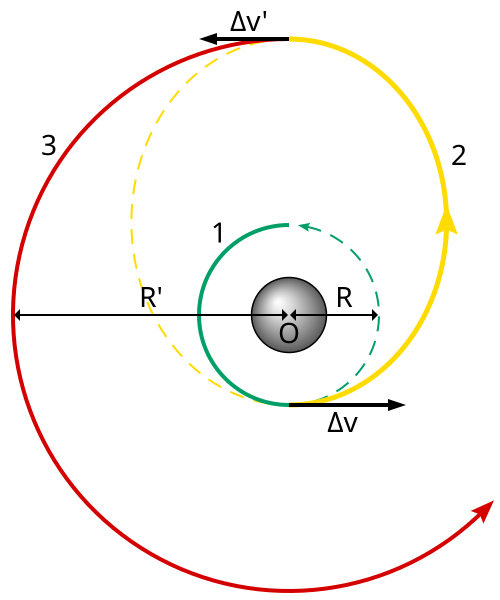
\includegraphics[width=0.33\textwidth]{images/Hohmann_transfer_orbit.svg.png}
    \caption{Hohmann Transfer Orbit}
\end{wrapfigure}
 A \textbf{Hohmann transfer orbit} is a mechanism by which an object moves
from a lower circular orbit to a higher circular orbit via an intermediary
elliptical orbit. The object travels from orbital radius $r_1$ to a higher
orbital radius $r_2$ on the diametrically opposite side.
So the semi-major
axis of the transfer ellipse is $ a = \frac{r_1 + r_2}{2} $ Our main goal is to find the velocity change when the object changes it's trajectory from a circular to an elliptical orbit. For this we will use the energy conservation equation for elliptical orbit.
First, for a circular orbit of radius $r$ around a mass $M$, the orbital speed is:

\begin{equation*}
    v_c = \sqrt{\frac{GM}{r}}
\end{equation*}

Applying conservation of energy at $r_1$ , we get the \textbf{vis-viva equation}:

\begin{equation*}
    \frac{1}{2}v_{ell}^2 - \frac{GM}{r_1} = -\frac{GM}{2a}
    \implies
    v_\mathrm{ell} = \sqrt{GM\!\left(\frac{2}{r_1} - \frac{1}{a}\right)}
\end{equation*}

Subtracting the circular orbital speed from the elliptical speed at $r_1$
gives the first velocity impulse:

\begin{equation*}
    \Delta v_1 = \sqrt{\frac{GM}{r_1}}
    \left(\sqrt{\frac{2r_2}{r_1 + r_2}} - 1\right)
\end{equation*}

Similarly, at $r_2$ the elliptical speed is:

\begin{equation*}
    v_\mathrm{ell} = \sqrt{GM\!\left(\frac{2}{r_2} - \frac{1}{a}\right)}
\end{equation*}

and the second velocity impulse, circularising the orbit at $r_2$, is:

\begin{equation*}
    \Delta v_2 = \sqrt{\frac{GM}{r_2}}
    \left(1 - \sqrt{\frac{2r_1}{r_1 + r_2}}\right)
\end{equation*}
% ----------------------------------------------------------------
\begin{tcolorbox}[colback=blue!5!white, colframe=blue!75!black,
                  title={Example: Geostationary Orbit to the Moon}]

A rocket of mass $m = 35{,}000~\mathrm{kg}$ orbits Earth at geostationary
altitude $h = 36{,}000~\mathrm{km}$. We wish to transfer it to the Moon's
orbit using a Hohmann transfer. Given:

\begin{itemize}
    \item $M_\oplus = 6\times10^{24}~\mathrm{kg}$
    \item $R_\oplus = 6{,}400~\mathrm{km}$
    \item Distance Earth--Moon: $r_2 = 384{,}400~\mathrm{km}$
    \item Lunar orbital period: $T_\mathrm{moon} = 27~\mathrm{days}$
    \item Exhaust velocity: $v_\mathrm{ex} = 2{,}500~\mathrm{m\,s^{-1}}$
    \item Both rocket and Moon orbit clockwise; Moon's orbit is treated as
          circular. Lunar gravity and non-circular effects are neglected.
\end{itemize}

\textbf{Tasks:}
\begin{enumerate}[label=\alph*)]
    \item How long does the semi-elliptical transfer take?
    \item What must the Moon--Earth--satellite angle be at the moment of
          the first burn?
    \item What percentage of the rocket's mass is expended?
\end{enumerate}

\end{tcolorbox}

\begin{tcolorbox}[colback=blue!5!white, colframe=blue!75!black,
                  title={Theory: Solution}]

\subsubsection*{(a)}

From Kepler's third law, $T^2 = \dfrac{4\pi^2}{GM}a^3 \equiv k^2 a^3$,
where:

\begin{equation*}
    k = \frac{2\pi}{\sqrt{GM_\oplus}}
      = 3.1398\times10^{-7}~\mathrm{s\,m^{-3/2}}
\end{equation*}

With $r_1 = h + R_\oplus = 42{,}400~\mathrm{km}$ and
$r_2 = 384{,}400~\mathrm{km}$:

\begin{equation}
    a = \frac{r_1 + r_2}{2} = 213{,}400~\mathrm{km}
\end{equation}

The transfer occupies half the full elliptical period:

\begin{equation*}
    T_\mathrm{transfer} = \frac{T}{2} = \frac{k}{2}\,a^{3/2}
    = 478{,}433~\mathrm{s} \approx 5.54~\mathrm{days}
\end{equation*}

\subsubsection*{(b)}

Were the Moon stationary, the required angle would be exactly
$180^\circ$. Since the Moon advances during the transfer, it must already
be $180^\circ$ ahead of its arrival point at the moment of the first burn.
The Moon travels through:

\begin{equation*}
    \theta_\mathrm{moon}
    = \frac{T_\mathrm{transfer}}{T_\mathrm{moon}}\times 360^\circ
    = \frac{5.54}{27}\times 360^\circ
    \approx 73.9^\circ
\end{equation*}

Therefore the required angle at the moment of the burn is:

\begin{equation*}
    \theta = 180^\circ - 73.9^\circ \approx 106^\circ
\end{equation*}



\end{tcolorbox}
\begin{tcolorbox}[colback=blue!5!white, colframe=blue!75!black,
                  title={Theory: Solution}]
                  \subsubsection*{(c)}

With $r_1 = 42{,}400~\mathrm{km}$ and $r_2 = 384{,}400~\mathrm{km}$:

\begin{align}
    \Delta v_1 &= \sqrt{\frac{GM_\oplus}{r_1}}
                 \left(\sqrt{\frac{2r_2}{r_1+r_2}}-1\right)
               = 1051.43~\mathrm{m\,s^{-1}} \\[6pt]
    \Delta v_2 &= \sqrt{\frac{GM_\oplus}{r_2}}
                 \left(1 - \sqrt{\frac{2r_1}{r_1+r_2}}\right)
               = 565.70~\mathrm{m\,s^{-1}}
\end{align}

Applying the  rocket equation
$|\Delta v| = v_\mathrm{ex}\ln(m_0/m_f)$ to each burn in sequence:

\begin{align}
    m_{f,1} &= m_0\exp\!\left(-\frac{|\Delta v_1|}{v_\mathrm{ex}}\right) \\[4pt]
    m_{f,2} &= m_{f,1}\exp\!\left(-\frac{|\Delta v_2|}{v_\mathrm{ex}}\right)
             = m_0\exp\!\left(-\frac{|\Delta v_1|+|\Delta v_2|}{v_\mathrm{ex}}\right)
\end{align}

The fractional mass loss is therefore:

\begin{equation}
    \frac{\Delta m}{m_0}
    = 1 - \exp\!\left(-\frac{|\Delta v_1|+|\Delta v_2|}{v_\mathrm{ex}}\right)
    = 1 - \exp\!\left(-\frac{1617.13}{2500}\right)
    \approx 47.6\%
\end{equation}

This may seem modest, but recall the conditions here are highly idealised.
\end{tcolorbox}
% ----------------------------------------------------------------
\section{Lagrange Points (L1 \& L2)}
\begin{figure}[h]
    \centering
    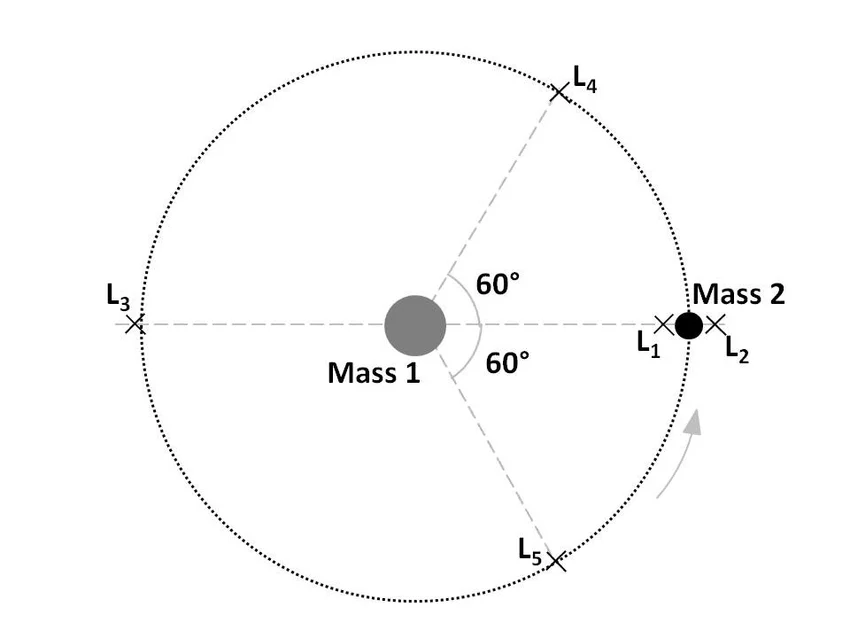
\includegraphics[width=0.4\textwidth]{images/lagrangepoints.png}
    \caption{Hohmann Transfer Orbit}
    \label{fig:hohmann}
\end{figure}
\noindent
Lagrange points are often nicknamed gravitational parking spots. It just means if we park our hypothetical spaceships in a single planet and star system, the spaceship will be stationary relative to the planet and star at that point\footnote{We're using an example of a planet star system for convenience, but it can be any two celestial object, where the smaller mass is orbiting a much larger mass, ideally in a circular motion}. But a key condition information about this is that, to an outside observer, the spaceship is actually rotating at the same angular velocity as the planet. There are exactly 5 such parking spots in such system. We're only going to elaborate on 2 for now.

\subsection*{Definitions}

\begin{itemize}
    \item $M_1$ = mass of the star
    \item $M_2$ mass of the planet
    \item $r$ = distance of the spacecraft from the planet
    \item $R$ = distance between the star and the planet
\end{itemize}

We further define the dimensionless variables(and $\omega$ which is very much not dimensionless):

\begin{equation*}
    x = \frac{r}{R}, \qquad
    \mu = \frac{M_2}{M_1 + M_2}, \qquad
    1 - \mu = \frac{M_1}{M_1 + M_2}, \qquad
    \omega^2 = \frac{G(M_1+M_2)}{R^3}
\end{equation*}

In systems where the secondary mass is much smaller than the primary (e.g., the Sun-Earth system), we assume that  $\mu \ll 1$ . Also, as the distance r is much smaller than R (we just know), we will also assume  $x \ll 1$. Though to note,  $\mu \ll x$.

\subsection*{$L_1$ point}

The $L_1$ point lies along the line connecting the star and planet, between
them. The hypothetical spacecraft is at distance $R - r$ from the star and $r$ from the
planet. Balancing the forces, we get.

\begin{equation*}
    \frac{GM_1 m}{(R-r)^2} - \frac{GM_2 m}{r^2} = m\omega^2(R-r)
\end{equation*}
Substitute the angular velocity $\omega^2 = \frac{G(M_1 + M_2)}{R^3}$:
\begin{equation*}
\frac{G M_1}{(R-r)^2} - \frac{G M_2}{r^2} = \frac{G(M_1 + M_2)}{R^3} (R - r)
\end{equation*}

Divide the entire equation by $\frac{G(M_1 + M_2)}{R^2}$:
\begin{equation*}
\frac{M_1/(M_1+M_2)}{(R-r)^2/R^2} - \frac{M_2/(M_1+M_2)}{r^2/R^2} = \frac{1}{R} (R - r)
\end{equation*}

Applying the definitions for $1-\mu$ and $\mu$, and substituting $x$:
\begin{equation*}
\frac{1-\mu}{(1-x)^2} - \frac{\mu}{x^2} = 1 - x
\end{equation*}

Using the Taylor expansion $(1-x)^{-2} \approx 1 + 2x$ for small $x$:
\begin{align*}
    (1-\mu)(1+2x) - \frac{\mu}{x^2} &\approx 1 - x \\
    1 + 2x - \mu - 2\mu x - \frac{\mu}{x^2} &\approx 1 - x \\
    3x^3 &= \mu x^2 + 2\mu x^3 + \mu
\end{align*}
Ignoring the higher order terms on the right hand side  as they are much smaller than $\mu$:

\begin{equation*}
    3x^3 = \mu
\end{equation*}

Which gives the final approximation for the distance to the $L_1$ point:

\begin{equation*}
    x = \sqrt[3]{\frac{\mu}{3}}
\end{equation*}
Which is the \textbf{hill radius}, we'll see shortly that L2 lies in the hill radius too

\subsection*{$L_2$ Point}

L2 point is still along the line of the star and the planet, but the point itself is beyond the planet. Thus the hypothetical spaceship is at a distance R+r from the star, and a distance r from the star. The force balance is:
\begin{equation*}
\frac{G M_1}{(R+r)^2} + \frac{G M_2}{r^2} = \omega^2 (R + r)
\end{equation*}

Through the same steps as the for L1, we get
\begin{equation*}
    \frac{1-\mu}{(1+x)^2} + \frac{\mu}{x^2} = 1 + x
\end{equation*}

Applying the approximation for $x \ll 1$ using $(1+x)^{-2} \approx 1 - 2x$:
\begin{align*}
    (1-\mu)(1-2x) + \frac{\mu}{x^2} &= 1 + x \\
   -3x^3 + 2\mu x^2 - \mu x^2 + \mu &= 0
\end{align*}

Ignoring the higher order terms ($x^3\mu$ and $x^2\mu$) as they are much smaller than $\mu$:

\begin{equation*}
    3x^3 = \mu
\end{equation*}

This yields the same first-order approximation as $L_1$:

\begin{equation*}
    x = \sqrt[3]{\frac{\mu}{3}}
\end{equation*}



\section{Tidal Force}

The name is pretty self-explanatory: it's the force which causes tides. We all know it is the Moon which causes the tides. And now we are gonna elaborate on that very topic.

The tidal force tries to create an acceleration, as all forces do. But the acceleration caused is actually the acceleration of that point (or the tides) relative to the planet \footnote{again it doesn't have to be between planet and its moon only, but rather between any two celestial bodies. Though, both masses can be similar, or one or the other can be larger.} as a whole caused by the moon only \footnote{we're ignoring the forces between the planet and the point mass because we're only interested in the moon's effect. }. Basically, tidal force is the additional force tides experience in a frame of reference where Earth is stationary and has no net acceleration. 

The variables we're going to need are:
\begin{itemize}
    \item $m_1$ = Mass of an object on Earth 
    \item $m_2$ = Mass of Earth
    \item $M$ = Mass of Moon
    \item $r$ = Radius of Earth
    \item $R$ = Distance between Earth and Moon centers
\end{itemize}

\subsection{Longitudinal Tidal Force}

For this case, we're going to calculate the tidal force on Earth at a point nearest to the moon. That point will be along the line connecting the Earth and the Moon. By the definition of relative acceleration, we get:

\begin{equation*}
a_{1/2} = a_1 - a_2 = \frac{GM}{(R-r)^2} - \frac{GM}{R^2} 
\end{equation*}

Factoring out the term $\frac{GM}{R^2}$:

\begin{equation*}
a_{1/2} = \frac{GM}{R^2} \left[ \left( 1 - \frac{r}{R} \right)^{-2} - 1 \right]
\end{equation*}

Using the Taylor expansion $(1+x)^n \approx 1 + nx$ for $x \ll 1$:

\begin{equation*}
a_{1/2} \approx \frac{GM}{R^2} \left[ \left( 1 + \frac{2r}{R} \right) - 1 \right] = \frac{2GMr}{R^3}
\end{equation*}

\bigskip
\[
\boxed{F_{\text{tidal}} = \frac{2GMm_1r}{R^3}}
\]


\begin{tcolorbox}[colback=blue!5!white,colframe=blue!75!black,title=Problem]
Compare the tidal force caused by the moon and the sun on a point mass on the surface of the earth
\end{tcolorbox}

\begin{tcolorbox}[colback=blue!5!white,colframe=blue!75!black,title=Solution]

Since the $G$, $m_1$ and $r$ terms cancel out, we have
\begin{equation*}
    \frac{F_s}{F_m} = \frac{M_s}{M_m} \cdot \left( \frac{R_m}{R_s} \right)^3 = 0.46
\end{equation*}
Thus the tidal force caused by the Moon is 2.2 times stronger than the Sun.

\end{tcolorbox}
\begin{tcolorbox}[colback=blue!5!white,colframe=blue!75!black,title=Problem]
Suppose an unfortunate astronaut fell into a black hole. The black hole has an event horizon radius of about $1R_{earth}. $
To begin the process of sphagettification, let's say, the astronaut would have to experience a tidal force on his head by around $F_t$ = 2000N force. If the man has a height of h = 180cm and mass of head $m_h$ = 5kg, at how many $1R_{\mathrm{Earth}}$ would the man begin sphagettification
\end{tcolorbox}
\begin{tcolorbox}[colback=blue!5!white,colframe=blue!75!black,title=Solution]

First of radius of event horizon, or the schwartzchild radius is 
\begin{align*}
    r = \frac{2GM}{c^2} \\
    M = \frac{R_{\mathrm{Earth}}c^2}{2G}
\end{align*}
And the tidal force,
\begin{align*}
   F_{\text{t}}= \frac{2GMm_1r}{R^3} = \frac{2GMm_h\frac{h}{2}}{r^3} = \frac{m_hR_{Earth}hc^2}{2r^3} \\
   r = \sqrt[3]{\frac{m_hR_{Earth}c^2}{2F_t}}
\end{align*}
In terms of Earth radius,
\begin{equation*}
     r = \frac{1}{R_{Earth}} \sqrt[3]{\frac{m_hR_{Earth}hc^2}{2F_t}} =  \sqrt[3]{\frac{m_hhc^2}{2F_tR_{Earth}^2}} \approx 1.8 R_{Earth}
\end{equation*}
\end{tcolorbox}



\subsection{General Tidal Force}

\begin{wrapfigure}{r}{0.45\textwidth}
    \centering
   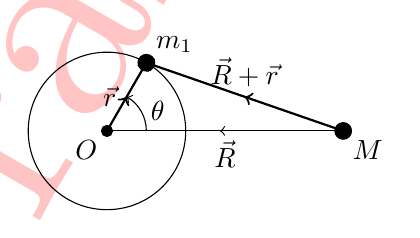
\begin{tikzpicture}
    % Main circle of radius r
    \draw (0,0) circle (1cm);
    
    % Centre dot
    \filldraw[black] (0,0) circle (2pt);
    
    % Label centre as O
    \node[below left] at (0,0) {$O$};

    % M dot to the right, R from centre
    \filldraw[black] (3,0) circle (3pt);
    \node[below right] at (3,0) {$M$};

    % m1 dot on the circumference at angle theta
    \filldraw[black] ({cos(60)},{sin(60)}) circle (3pt);
    \node[above right] at ({cos(60)},{sin(60)}) {$m_1$};

    % Vector from O to m1 with mid-arrow, labelled vec{r}
    \draw[->, thick, postaction={decorate, decoration={
        markings, mark=at position 0.5 with {\arrow{>}}
    }}] (0,0) -- ({cos(60)},{sin(60)}) 
        node[midway, left] {$\vec{r}$};

    % Vector from M to m1 with mid-arrow, labelled vec{R}
    \draw[->, thick, postaction={decorate, decoration={
        markings, mark=at position 0.5 with {\arrow{>}}
    }}] (3,0) -- ({cos(60)},{sin(60)}) 
        node[midway, above] {$\vec{R}+\vec{r}$};

    % Vector from O to M with mid-arrow only (no tip), labelled R
    \draw[postaction={decorate, decoration={
        markings, mark=at position 0.5 with {\arrow{<}}
    }}] (0,0) -- (3,0) node[midway, below] {$\vec{R}$};

    % Angle arc for theta
    \draw[->] (0.5,0) arc (0:60:0.5cm) node[midway, right] {$\theta$};
\end{tikzpicture}
    \caption{Mass $m_1$ on circle of radius $r$, and mass $M$ at distance $R$}
\end{wrapfigure}
If we want a general equation for tidal force, that is, we want an equation of tidal force on all points of the surface of the earth. Such that if we put Earth on the origin, Moon at a distance $R$ along the $x$-axis, the point will lie on an angle $\theta$ with respect to the $x$-axis (and the moon).

Now, the equation will stand as,
\[
\vec{a}_{1/2} = \vec{a}_1 - \vec{a}_2 
= -\frac{GM(\vec{R}+\vec{r})}{|\vec{R}+\vec{r}|^3} - \frac{GM\,\hat{i}}{R^2}
\]
(using the vector form of Newton's law of gravitation)

Again we know $|\vec{a} + \vec{b}| = \sqrt{a^2 + b^2 + 2ab\cos\theta}$

Thus,
\[
= \frac{-GM\left[(-R\,\hat{i} + r\cos\theta\,\hat{i} + r\sin\theta\,\hat{j})\right]}{(R^2 + r^2 + 2Rr\cos\theta)^{3/2}} - \frac{GM\,\hat{i}}{R^2}
\]

\[
= \frac{-GM\left[(-R + r\cos\theta)\,\hat{i} + r\sin\theta\,\hat{j}\right]}{R^3\!\left(1 + \dfrac{r^2}{R^2} + \dfrac{2r}{R}\cos\theta\right)^{3/2}} - \frac{GM\,\hat{i}}{R^2}
\]

\[
= \frac{-GM\left[(-R + r\cos\theta)\,\hat{i} + r\sin\theta\,\hat{j}\right]}{R^3}\left(1 + \frac{3r}{R}\cos\theta\right) - \frac{GM\,\hat{i}}{R^2}
\]
(by Taylor expansion, removing higher-order terms)

\bigskip
\noindent\textbf{Taking the $x$-component only:}
\begin{align*}
(a_{1/2})_x 
&= \frac{-GM(-R + r\cos\theta)}{R^3}\!\left(1 + \frac{3r}{R}\cos\theta\right) - \frac{GM}{R^2} \\[6pt]
&= \frac{GM}{R^2} - \frac{GMr\cos\theta}{R^3} + \frac{3GMr\cos\theta}{R^3} + \frac{3GMr^2\cos^2\theta}{R^4} - \frac{GM}{R^2} \\[6pt]
&= \frac{2GMr\cos\theta}{R^3}
\end{align*}
(cancelling equal and opposite terms, ignoring higher-order terms like $r^2/R^4$)

\bigskip
\noindent\textbf{Taking the $y$-component only:}
\begin{align*}
(a_{1/2})_y 
&= \frac{-GM\,r\sin\theta}{R^3}\!\left(1 + \frac{3r}{R}\cos\theta\right) \\[6pt]
&= -\frac{GMr\sin\theta}{R^3} - \frac{3GMr^2\sin\theta\cos\theta}{R^4} \\[6pt]
&= -\frac{GMr\sin\theta}{R^3}
\end{align*}
(ignoring the higher-order $r^2/R^4$ term)

\bigskip
\noindent Therefore, the general tidal force vector is:
\[
\boxed{\vec{F}_{tidal} = \frac{GMm_{1}r}{R^3}\left(2\cos\theta\,\hat{i} - \sin\theta\,\hat{j}\right)}
\]

\begin{tcolorbox}[colback=blue!5!white,colframe=blue!75!black,title=Problem]
At what angle will the tidal force be maximum
\end{tcolorbox}

\begin{tcolorbox}[colback=blue!5!white,colframe=blue!75!black,title=Solution]
Letting $\frac{GMm_1r}{R^3}=k$,
\begin{align*}
    \abs{F_{tidal}} &=\sqrt{4k^2cos^2\theta+k^2sin^2\theta} \\
        &= k\sqrt{1+3cos^2\theta}
\end{align*}
    So, we need to maximize the term $1+3cos^2\theta$
    Thus,
\begin{align*}
    f'(\theta) = -6cos\theta sin\theta = -3sin2\theta = 0 \\
\end{align*}
\begin{equation*}
    \text{Thus } \theta=0^\circ, 90^\circ,180^\circ, 270^\circ
\end{equation*}
\begin{align*}
    f(\theta) &= 4 , \text{ when } \theta=0^\circ, 180^\circ \\
    f(\theta) &= 1 , \text{ when } \theta=90^\circ, 270^\circ
\end{align*}
So, tidal force maximizes at 0 and 180 degrees in theory
\end{tcolorbox}
\newpage
\subsection{Roche limit}
In relation to our previous topic, tidal forces, Roche limit is a radius, below which any other celestial object can no longer maintain it's shape. What happens then is the celestial object disintegrates, as the tidal force caused by the other celestial object exceeds the gravitational force of it's own. 
\\
So naturally we can try equating the two forces, \footnote{We are taking the longitudinal tidal force equation, as tidal force is strongest in the longitudinal direction}
Let,
\begin{align*}
    F_t &= F_g \\
    \frac{2GMm_1x}{R^3} &= \frac{Gm_2m_1}{x^2} \\
    2\frac{x^3}{R^3} &= \frac{m_2}{M} = \frac{x^3 \rho_2}{r_M^3 \rho_M} \\
    R &= r_M \sqrt[3]{2\frac{\rho_M}{\rho_2}} \\
    R &\approx 1.44 r_M \sqrt[3]{\frac{\rho_M}{\rho_2}} 
\end{align*}


\begin{center}
    
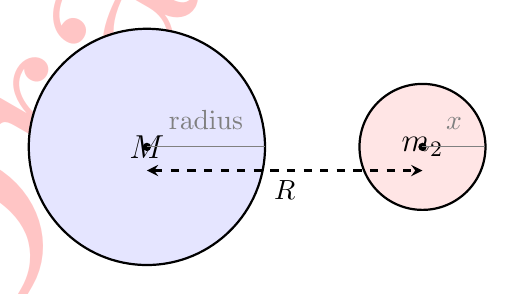
\begin{tikzpicture}

  % Parameters
  % First circle: radius R1 = 2.5, centered at origin
  % Second circle: radius R2 = 1.2, center at distance d = 5 from first circle's center

  \def\Rone{1.5}   % radius of first circle
  \def\Rtwo{0.8}   % radius of second circle (smaller)
  \def\dist{3.5}     % distance between centers

  % --- First Circle ---
  \draw[thick, fill=blue!10] (0,0) circle (\Rone);
  \node at (0,0) [font=\large\bfseries] {$M$};
  % Center dot
  \fill (0,0) circle (1.5pt);

  % --- Second Circle ---
  \draw[thick, fill=red!10] (\dist,0) circle (\Rtwo);
  \node at (\dist,0) [font=\large\bfseries] {$m_2$};
  % Center dot
  \fill (\dist,0) circle (1.5pt);

  % --- Distance annotation (R between centers) ---
  \draw[<->, >=stealth, thick, dashed]
    (0, -0.3) -- (\dist, -0.3)
    node[midway, below] {$R$};

  % --- Radius labels ---
  % First circle radius
  \draw[-, gray] (0,0) -- (\Rone, 0)
    node[midway, above, gray] {};
  \node[above, gray] at (\Rone/2, 0.1) {radius};

  % Second circle radius label (x)
  \draw[-, gray] (\dist,0) -- (\dist+\Rtwo, 0);
  \node[above, gray] at (\dist+\Rtwo/2, 0.1) {$x$};
\end{tikzpicture}
\\[1EM]
Mass of $M$, and at a distance R there's mass of $m_2$ of radius x. Mass $m_1$ can be assumed to be somewhere on the surface of $m_2$ along the longitudinal axis


\\[2EM]

\end{center}
\begin{thebibliography}{99}

    % --- Image References ---
    \subsection*{Image References}

    \bibitem{hohmann}
    Wikimedia Commons.
    \textit{Hohmann Transfer Orbit}.
    [Online]. Available:
    \url{https://en.wikipedia.org/wiki/Hohmann_transfer_orbit}

    \bibitem{lagrange}
    Wikimedia Commons.
    \textit{Lagrange Points}.
    [Online]. Available:
    \url{https://en.wikipedia.org/wiki/Lagrange_point}

    % --- Text References ---
    \subsection*{References}

    \bibitem{ref1}
    Hannu Karttunen,
    \textit{Fundamental Astronomy}.
    

    \bibitem{ref2}
    David Morin,
    \textit{Introduction to Classical Mechanics}.
   

\end{thebibliography}
\end{document}